% -*-coding: utf-8;-*-
%\chapter{Нейросетевое управление в нестационарных условиях}

Во многих случаях система управления проектируется исходя из
предположения о постоянстве её параметров, однако в реальном мире нет
ничего неизменного.  Элементы системы управления со временем
изнашиваются, условия внешней среды меняются, в процессе
функционирования возможны случайные деструктивные воздействия,
меняющие характеристики элементов, например, аварии.  Эти процессы
иногда можно предвидеть, но всегда трудно точно описать, поскольку они
носят вероятностный характер.

Фактор износа элементов системы можно учеть, расчитав срок их
эксплуатации и проводя превентивную замену давно работающего элемента
на новый с номинальными характеристиками.  Вариации условий внешней
среды можно заложить в исходную модель в качестве возмущающих
воздействий или просто на модели убедиться в сохранении устойчивости и
качества функционирования системы управления во всем диапазоне
возможных отклонений внешних условий.  Эти решения дают
удовлетворительный результат, однако их отличает то, что они
неоптимальны, а значит, приводят к экономическим потерям: замене по
регламенту вполне ещё исправных элементов, неоптимальная работа
контура управления в течение длительных периодов отличия внешних
условий от расчетных.

Случайные воздействия на элементы системы автоматического управления
совершенно непредсказуемы и по вероятности их возникновения и по
производимому эффекту.  Случаи катастофических изменений, как правило,
легко отслеживаются и исправляются заменой вышедших из строя
элементов.  Однако, небольшие изменения вызываются лишь отклонения в
штатном функционировании системы, малозаметные, но могущие привести к
серьезным последствиям: непредусмотренному повышенному износу, браку,
сбоям в других связанных системах управления.

Вышеперечисленные факторы однозначно свидетельствуют о важности
развития методов управления, адаптированным к нестационарному
поведению объекта.  В частности, наиболее целесообразно рассмотреть
случай ступенчатого изменения свойств объекта.  Рассмотрим
нейросетевые методы для управления нестационарным объектов.

\begin{figure}[h]
\centering
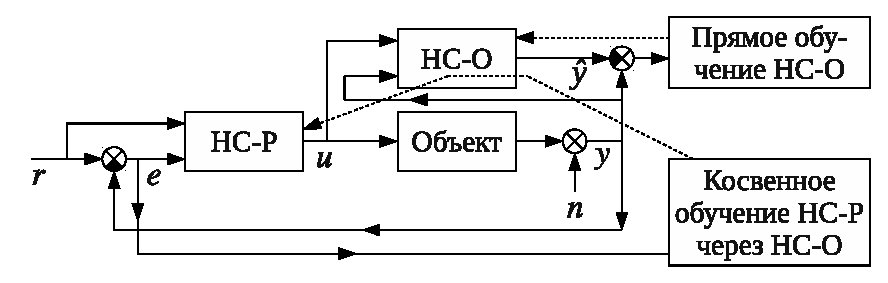
\includegraphics{permanent_adoption_rus}
\caption{Контур управления в режиме постоянной адаптации.}
\label{fig:permanent_adoption_loop}
\end{figure}

\begin{figure}[h]
\centering
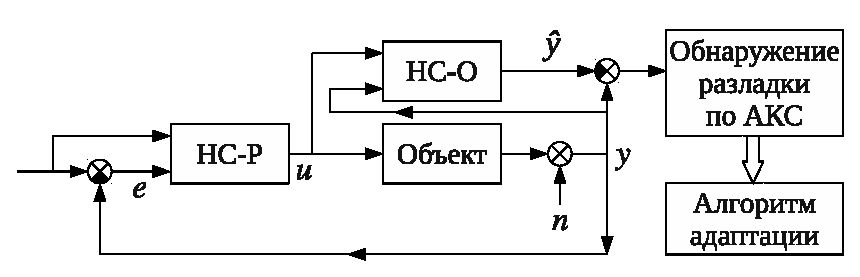
\includegraphics{steady_state_rus}
\caption{Контур управления в стационарном режиме.}
\label{fig:steady_state_loop}
\end{figure}

\begin{figure}[h]
\centering
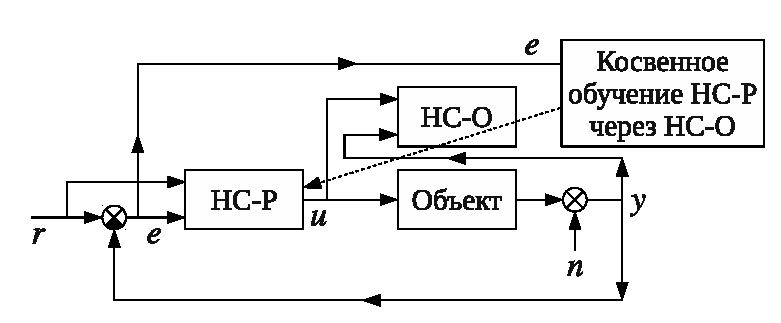
\includegraphics{modified_adoption_rus}
\caption{Контур управления в режиме адаптации к разладке.}
\label{fig:permanent_adoption_loop}
\end{figure}

\section{Постановка задачи}

Существуют различные
подходы к решению данной задачи, в том числе и получивший в последнее
время достаточно большое распространение подход, основанный на
использовании в системах управления искусственных нейронных сетей
(ИНС) [1,2]. При реализации соответствующих самонастраивающихся
алгоритмов управления (в том числе нейросетевых) в первую очередь
исследуются вопросы оценки качества управления в переходных режимах и
обеспечения устойчивости системы при самонастройке. В то же время
фактически игнорируется проблема экономичности и минимизации потерь от
процесса подстройки регулятора: этот процесс, как правило, просто
реализуется постоянно вне зависимости от того, изменились ли свойства
объекта управления или нет. Задача стоит особенно остро для ситуации,
когда уставка и внешняя помеха имеют случайный характер.  Целью данной
работы является разработка нейросетевого оптимального регулятора,
предназначенного для управления нестационарным объектом и
обеспечивающего минимизации потерь от самонастройки, а также методики
его синтеза. Указанная минимизация достигается путем реализации
процесса самонастройки только при реальной на то необходимости.


Предметом рассмотрения является самонастраивающаяся нейросетевая
система автоматического управления (НСАУ) объектом. В исходном
варианте она содержит нейросетевой регулятор НС-Р и нейросетевую
модель объекта управления НС-О. Для нестационарного объекта
традиционно осуществляется непрерывная корректировка НС-О и – с ее
помощью – подстройка НС-Р. В условиях, когда и уставка и помеха
являются случайными процессами, это может повлечь за собой
существенное увеличение ошибки управления. Для устранения данного
недостатка предлагается ввести в НСАУ дополнительный элемент,
предназначенный для обнаружения момента изменения свойств объекта
управления (ОУ). Тогда процедура подстройки НС-Р и НС-О будет
исполняться только после того, как этим элементом будет обнаружено
существенное систематическое расхождение в статистических свойствах
сигналов на выходах объекта и НС-О, т.е. когда ошибка идентификации
объекта с помощью НС-О значимо возросла. В качестве средства
обнаружения такого расхождения (``разладки'') предложено использовать
классический алгоритмом кумулятивных сумм (АКС) [3].

Структурная схема модернизированной НСАУ с дополнительным элементом
АКС представлена на рис.1. Синтез подобной НСАУ сопряжен со
значительными трудностями. Для их преодоление предлагается
соответствующая методика, позволяющая в конечном итоге получить НСАУ,
оптимальную в смысле минимума общей среднеквадратической ошибки
управления нестационарным объектом и организовать ее реальное
функционирование.

\section{Метод постоянной адаптации}
\section{Метод адаптации по обнаружению разладки}
\subsection{Первоначальный синтез}

в первую очередь включает в себя выбор архитектуры нейростевой модели
объекта и нейрорегулятора. Исходя из идеи максимального упрощения
реализации, для их построения предлагается использовать многослойные
персептроны [1,4] с сигмоидальной функцией активации всех нейронов за
исключением нейрона последнего слоя, которая может быть линейной.

Нейронная сеть модели объекта управления (рис.2а) в каждый текущий
момент дискретного времени k получает на вход управляющее воздействие
регулятора uk , наблюдаемый выход объекта управления yk, а также их
значения в предыдущие моменты времени uk-1, uk-2, …, uk-Du, yk-1,
yk-2, …, yk-Dy.  Динамический характер отклика нейронной сети,
отражающий динамические свойства объекта управления, обеспечивается в
данном случае не за счет внутренней памяти, характерной для сетей с
обратными связями, а за счет использования предистории, хранимой вне
сети.  Выходом сети является предполагаемый выход объекта управления
ŷk+1 в момент времени k+1, т.е. нейросетевая модель настраивается для
предсказания поведения объекта на основе предистории значений
управляющих сигналов и наблюдения за объектом (вместе с
помехой). Данными для обучения сети НС-О являются ряды {uk}N и {yk}N,
составляющие обучающую выборку объема N, причем наблюдаемый выход ОУ
используется как на входе нейронной сети, так и в качестве образца на
выходе.  Целью обучения для ОУ с одним наблюдаемым выходом является
построение отображения (Du+Dy)-мерного множества, задающего входной
вектор, на одномерное множество выходных значений: UDuYDyY.

(а)

(б)
Рис.2. Структура нейронных  сетей НС-О (а) и НС-Р (б).

Задача выбора числа входов для ИНС типа многослойного персептрона в
рассматриваемом случае моделирования динамического объекта не имеет
строго формализованного решения. Для выработки некоторых рекомендаций
по выбору количества входов u и y — Du и Dy соответственно — был
проведен вычислительный эксперимент, в котором определялось влияние Du
и Dy на качества обучения НС-О.  В эксперименте нейронная сеть
фиксированной архитектуры (два скрытых слоя с 8 и 3 нейронами в
каждом) обучалась предсказанию выхода инерционного ОУ на обучающей
выборке фиксированной длины N=500 в течение 400 эпох (использовалось
пакетное обучение по методу BPE [4]).  Сигналом u выступал белый шум,
распределенный по гауссовскому закону с параметрами и .  В канале
наблюдения присутствовала аддитивная помеха, также нормально
распределенная с и .  В разных сериях экспериментальных данных ОУ
выступал с различными значениями параметра инерционности d: от 0.1 до
0.9 с шагом 0.1.  Это соответствует времени установления переходного
процесса от 0.43 до 9.49 дискретных отсчетов времни.  Число входов
НС-О варьировалась от 1 до 4 (по Du и Dy независимо).

Анализ результатов показал:
\begin{itemize}
\item Соблюдение условия Du≤Dy приводит к меньшей ошибке (в 2-3 раза).
\item При фиксированном Dy>1 ошибка увеличивается с увеличением инерционности объекта.
\end{itemize}

Из общих соображений можно также предположить, что:
\begin{itemize}
\item Предсказание объекта с чистым запаздыванием требует длины
  истории Dy, не меньшей времени запаздывания.
\item Чем выше порядок многочлена в знаменателе передаточной функции
  объекта G*(z), тем длиннее должна быть история Dy.
\end{itemize}

Аналогичное исследование было проведено и для НС-Р. В результате
экспериментов по выбору номенклатуры входов нейросетевого регулятора
наилучшие результаты (самая быстрая скорость обучения; наименьшая
ошибка управления) оказались у пары уставка (rk) - ошибка
управления (ek) (рис. 2б).

Первоначальная настройка нейросетевого регулятора и построения
нейросетевой модели динамического объекта, а также АКС производится с
помощью известных процедур, достаточно подробно изложенных, например,
в [2-4].

\subsection{Формирование обучающей выборки и настройка НС-О}

в данном случае имеет свою специфику, что проявляется в выборе длины
обучающей выборки N и в способе ее формирования. Стандартный подход
использования обучающей выборки постоянной длины в данном случае
нецелесообразен. Дело в том, что подстройка НС-О, должна производиться
каждый раз при появлении сигнала о наличии разладки. Начиная с этого
момента можно считать установленным, что НСАУ находится не в
оптимальном режиме, и желательно минимизировать время этого
нахождения. Хотя понятно, что чем больше длина обучающей выборки для
подстройки НС-О, тем, в общем, качественнее будет настроена НС-О и,
соответственно, НС-Р, однако затягивание процесса формирования
обучающей выборки крайне нежелательно. Поэтому предлагается
использовать в качестве такой выборки элементы {uk}N и {yk}N ,
зафиксированные на интервале от начала запуска последней
контролирующей процедуры АКС t0 до момента t1 выработки сигнала о
наличии разладки (обозначим их количество ) плюс аналогичных значений,
имевших место до момента t0.  Поскольку значение t1 является случайной
величиной, в результате будет получена обучающая выборка случайной
длины . Далее на полученной выборке осуществляется начальный цикл
подстройки НС-О вне контура управления (в машинном времени).

\subsection{Подстройка НС-Р в контуре управления}
\subsection{Настройка АКС для обнаружения разладки}
\section{Имитационное моделирование}
\section{Выводы}
